\PassOptionsToPackage{utf8}{inputenc}
\documentclass{bioinfo}
\usepackage{xspace}
\usepackage[ruled,vlined,linesnumbered]{algorithm2e}
\usepackage[binary-units=true]{siunitx}
\usepackage{cleveref}
\usepackage{todonotes}
\usepackage{mathtools}

\newcommand{\ie}{i.\,e.\@\xspace}
\newcommand{\eg}{e.\,g.\@\xspace}
\newcommand{\cf}{cf.\@\xspace}
\newcommand{\wrt}{w.\,r.\,t.\@\xspace}
\newcommand{\ALG}{\ensuremath{\mathtt{ALG}}\xspace}
\newcommand{\dbb}[1]{{\color{blue}/******DBB:

#1

*********/
}}

\copyrightyear{2015} \pubyear{2015}

\access{Advance Access Publication Date: Day Month Year}
\appnotes{Original Paper}

\begin{document}
\firstpage{1}

\subtitle{Systems Biology}

\title[Robust disease module mining]{ROBUST: Robust disease module mining via enumeration of  prize-collecting Steiner trees} 
\author[Bernett \textit{et~al}.]{%
Judith Bernett\,$^{\text{\sfb 1,}*}$, % 
Dominik Krupke\,$^{\text{\sfb 2,}*}$, % 
Sepideh Sadegh\,$^{\text{\sfb 1}}$, % 
Jan Baumbach\,$^{\text{\sfb 3,4}}$, % 
S\'andor P. Fekete\,$^{\text{\sfb 2}}$, % 
Tim Kacprowski\,$^{\text{\sfb 5,6}}$, % 
Markus List\,$^{\text{\sfb 1}}$, % 
and David B. Blumenthal\,$^{\text{\sfb 7,}\dagger}$}



\address{%
$^{\text{\sf 1}}$Chair of Experimental Bioinformatics, TUM School of Life Sciences, Technical University of Munich, Freising, Germany \\
$^{\text{\sf 2}}$Institute of Operating Systems and Computer Networks, Technical University of Brunswick, Brunswick, Germany\\
$^{\text{\sf 3}}$Chair of Computational Systems Biology, University of Hamburg, Hamburg, Germany\\
$^{\text{\sf 4}}$Department of Mathematics and Computer Science, University of Southern Denmark, Odense, Denmark\\
$^{\text{\sf 5}}$Division of Data Science in Biomedicine, Peter L. Reichertz Institute for Medical Informatics, Technical University of Brunswick and Hannover Medical School, Brunswick, Germany\\
$^{\text{\sf 6}}$Braunschweig Integrated Centre of Systems Biology (BRICS), Brunswick, Germany\\
$^{\text{\sf 7}}$Department Artificial Intelligence in Biomedical Engineering, Friedrich-Alexander University Erlangen-Nürnberg, Erlangen, Germany}

\corresp{%
$^\ast$Equally contributing first authors.\\
$^\dagger$To whom correspondence should be addressed.}

\history{Received on XXXXX; revised on XXXXX; accepted on XXXXX}
\editor{Associate Editor: XXXXXXX}

\abstract{\textbf{Motivation:} Disease module mining methods (DMMMs) mine molecular networks\,---\,usually, protein-protein interaction (PPI) networks\,---\,for subgraphs that constitute candidate disease mechanisms. Various DMMMs have been presented during the last years, using very different mathematical models. However, irrespectively of the employed models, most DMMMs share the problem that they include non-deterministic steps in their workflows, \ie, that the computed subnetworks vary when running the DMMMs multiple times on equivalent input. This lack of robustness has a negative effect on the trustworthiness of the obtained subnetworks and is hence detrimental for the wide-spread adoption of DMMMs in the biomedical sciences.\\
\textbf{Results:} To overcome this problem, we present a new DMMM called ROBUST (\textbf{robu}st disease module mining via enumeration of prize-collecting \textbf{S}teiner \textbf{t}rees). In a large-scale empirical evaluation, we show that, unlike all tested competitors, ROBUST achieves almost perfect robustness. Moreover, in most settings, ROBUST outperforms existing DMMMs in terms of functional relevance of the produced subgraphs, measured via KEGG gene set enrichment scores and overlap with DisGeNET disease genes.\\
\textbf{Availability:} A Python 3 implementation and scripts to reproduce the results reported in this paper are available on GitHub: \href{https://github.com/bionetslab/robust}{https://github.com/bionetslab/robust}, \href{https://github.com/bionetslab/robust}{https://github.com/bionetslab/robust-eval}.\\
\textbf{Contact:} \href{mailto:david.b.blumenthal@fau.de}{david.b.blumenthal@fau.de}\\
\textbf{Supplementary information:} Supplementary data are available at \textit{Bioinformatics} online.}

\maketitle

\section{Introduction}

Over the last decades, high-throughput technologies and genome-wide association studies have generated an immense amount of omics data, enabling the generation of widely ramified and detailed interaction networks. Motivated by the possibility to uncover the pathobiology of complex diseases, the field of network medicine has emerged, which tries to untangle these connections and pinpoint the source of certain clinical pictures. Because of the nature of the data, this field faces various challenges. Most importantly, gene expression data are often noisy and overdetermined and mutations of healthy pathways typically have a cascading effect, leading to hundreds of differentially expressed genes. Additionally, not all of the genes triggering a certain disease might be differentially expressed in an experiment because the expression profiles are just a snapshot of the state of a cell. Therefore, the discovery of disease genes using simple statistical tests is infeasible. Consequently, disease module mining methods (DMMMs) are developed in the field of network medicine, which combine analyses of gene expression profiles with mining of prior knowledge encoded in protein-protein interaction (PPI) networks. 

DMMMs try to identify significantly enriched subnetworks by projecting the expression data on the PPI networks. Since solving the underlying mathematical models to optimality is typically NP-hard \citep{np_ideker2002}, heuristic algorithms are used in practice, where different weight and scoring metrics are applied to the network components. Using these algorithms, subnetworks can be identified that are significantly associated with a certain disease, even when some of the individual nodes have a negligible score. Various DMMMs have been proposed in the past years (see \cite{Batra2017-po}, \cite{Lazareva2021-jb}, and \cite{amim_lazareva2021} for recent surveys). They have enabled new insights into complex diseases like type-2 diabetes \citep{diabetes_sharma2018,diabetes_fernandez2019}, pulmonary arterial hypertension \citep{pulmonary_samokhin2018}, coronary heart disease \citep{coronary_wang2018}, and asthma \citep{asthma_sharma2015}.

Despite these success stories, existing DMMMs are known to be subject to several limitations. For instance, \cite{domino_levi2021} have shown that most DMMMs do not fully exploit the information contained in the gene expression data. \cite{amim_lazareva2021} have demonstrated that most DMMMs mainly learn from the node degrees rather than from the biological knowledge encoded in the edges of the PPI networks. 

In this paper, we draw attention to an additional issue which has not been addressed yet: Existing DMMMs lack of robustness and are subject to random bias. The reason for this is that all DMMMs we are aware of include non-deterministic steps in their workflows, although this aspect is often not explicitly mentioned and sometimes hidden in the storage order of the input data. This leads to variations in the resulting subnetworks when DMMMs are run multiple times on equivalent input. This lack of robustness is a major limitation, because reliable output is crucial to achieve a widespread adoption of DMMMs in the biomedical research community. 

To address this issue, we here present a new DMMM called ROBUST, short for \textbf{robu}st disease module mining via enumeration of prize-collecting \textbf{S}teiner \textbf{t}rees. ROBUST proceeds in two steps. Firstly, multiple pairwise dissimilar candidate disease modules (modeled via close-to-optimal prize-collecting Steiner trees) are enumerated. Next, the subnetwork induced by nodes that are contained in many of them is returned.

A large-scale evaluation on data for \num{903} diseases shows that, unlike all tested competitors, ROBUST achieves almost perfect robustness. Moreover, tests on gene expression data for amyotrophic lateral sclerosis (ALS), non-small cell lung cancer (LC), ulcerative colitis (UC), Chron’s disease (CD), and Huntington’s disease (HD) demonstrate that, in most settings, ROBUST outperforms its competitors in terms of functional relevance of the returned modules, which we measured via KEGG \citep{kegg_kanehisa2016} gene set enrichment \wrt known disease-associated pathways and overlap with DisGeNET \citep{disgenet_pinero2020} disease genes. Finally, a case study in \textcolor{red}{[SPECIFY DISEASE]} yields \textcolor{red}{[SUMMARIZE FINDINGS]}.


%In this paper, we focus on the algorithms DIAMOnD \citep{diamond_ghiassian2015}, DOMINO \citep{domino_levi2021}, and MuST \citep{covex_sadegh2020}
%Various algorithms have been proposed for identifying disease modules including DIAMOnD (\cite{diamond_ghiassian2015}), DOMINO (\cite{domino_levi2021}), MuST (multi-Steiner tree algorithm, \cite{covex_sadegh2020}), %from the DOMINO paper:
%jActiveModules (\cite{np_ideker2002}), BioNet (\cite{bionet_beisser2010}), HotNet2 (\cite{hotnet2_leiserson2015}), NetBox (\cite{netbox_cerami2010}), KeyPathwayMiner (\cite{keypathwayminer_alcaraz2011, keypathway_baumbach2012, keypathwayminer_alcaraz2014, keypathwayminerweb_list2016}), %from the AMIM paper:
%ClustEx2 (\cite{clustex2_ding2018}), COSINE (\cite{cosine_ma2011}), GiGA (\cite{giga_breitling2004}), GXNA (\cite{gnax_nacu2007}), GrandForest (\cite{grandforest_larsen2020}) and NetCore (\cite{netcore_barel2020}). Of these algorithms, DOMINO, DIAMOnD, MuST, ClustEx2 and NetBox require a binarized input (seed genes that were e.g. significant in the differential expression analysis) while the other methods project gene expression or mutation data on the PPI network. 
%
%In their benchmark analysis, Levi \textit{et al.} have proven that most DMMMs learn mainly from network structure and not from the actual gene expression data. By permuting the gene expression measurements and comparing the resulting set of enriched GO terms with the set computed from the real activity scores, they showed that the overlap of the sets was high for most methods.  \cite{amim_lazareva2021} have additionally demonstrated that most DMMMs do not produce significantly more biologically meaningful disease modules when they are run on permuted networks that preserve the node degrees. An additional issue that has not been explicitly addressed yet, is the robustness of the methods. Most DMMMs include non-deterministic steps in their workflows, leading to variations in the resulting subnetworks when they are run multiple times on equivalent input. Furthermore, we hypothesized that the underlying heuristics are influenced by the order that the network was read into memory.  Because it is important to have a reliable output in order to achieve a widespread adoption of DMMMs in the biomedical research community, we present a new method, ROBUST, short for \textbf{robu}st disease module mining via enumeration of price-collection \textbf{S}teiner \textbf{t}rees. %TODO: High-level description of how ROBUST addresses this problem
%
%We decided to compare our novel approach to DIAMOnD, DOMINO, MuST and a randomized version of MuST. Only methods with binary input were chosen since it was shown that they generally performed better because they were not as susceptible to noise (\cite{domino_levi2021}). DIAMOnD was selected since it is arguably the most widely used DMMM (\cite{diamond_popular_cui2019}). In the study by Lazareva \textit{et al}, DIAMOnD is outperformed by the recently introduced tool DOMINO. MuST and the randomized version of MuST (R-MuST) were included since they consitute the point of departure for the ROBUST method. %TODO more?    
%
%In a large-scale empirical evaluation, we show that, unlike all tested competitors, ROBUST achieves almost perfect robustness. Moreover, in most settings, ROBUST outperforms  existing  DMMMs  in  terms  of  functional  relevance  of  the  produced  subgraphs, measured via KEGG gene set enrichment w. r. t. known disease-associated pathways and overlap with DisGeNet disease genes.


\section{Methods}

\subsection{Modeling disease modules via relaxed Steiner trees}

Two strategic decisions have to be made when designing a new DMMM. Firstly, one has to decide which input should be expected. In addition to a PPI network, existing DMMMs use various types of input data such as normalized expression data \citep{gnax_nacu2007,cosine_ma2011,grandforest_larsen2020}, gene scores \citep{Reyna2018-ti,netcore_barel2020}, sorted lists of genes \citep{giga_breitling2004}, indicator matrices of differentially expressed genes \citep{keypathwayminerweb_list2016}, or binary input in the form of sets of disease-associated or differentially expressed seed genes \citep{diamond_ghiassian2015,clustex2_ding2018,covex_sadegh2020,domino_levi2021}. For ROBUST, we chose the latter option for the following reasons:
\begin{itemize}
\item Sets of disease-associated seed genes are very user-friendly input. They can be computed via standard differential gene expression analysis or be obtained from public databases such as OMIM \citep{Amberger2019-mp} or DisGeNET \citep{disgenet_pinero2020}, which provide disease-gene associations obtained from genome-wide association studies (GWAS). 
\item \cite{domino_levi2021} have shown that DMMMs using seed sets as input tend to outperform DMMMs operating on non-binary input data.
\end{itemize}

The second question is how the disease module mining problem should be modeled mathematically. Here, we chose minimum-weight relaxed (relaxation is explained below) Steiner trees. Recall that a minimum-weight Steiner tree for a weighted network $G=(V,E,w)$ and a set of seed nodes $S\subseteq V$ is a tree $T=(V_T,E_T)$ with $S\subseteq V_T\subseteq V$, $E_T\subseteq E$, and minimum total weight $\sum_{e\in E_T}w(e)$. Computing minimum-weight Steiner trees is NP-hard, but efficient approximation algorithms exist, \eg, the classical $2$-approximation algorithm by \cite{kou:1981aa}.

From a biological point of view, using minimum-weight Steiner trees to model the disease module mining problem is promising. Functionally related genes or proteins tend to be close to each other in the molecular interaction network and it could be shown that pairwise shortest paths of known disease genes show a considerable left shift in their distribution compared to the random expectation \citep{Menche2015-bp}. A reasonable hypothesis in network medicine is hence that the shortest paths between these disease genes overlap with causal molecular pathways \citep{Barabasi2011-yb}. Since minimum-weight Steiner trees can be viewed as generalizations of shortest paths to settings where more than two endpoints are given, a disease module constructed using minimum-weight Steiner trees can be expected to cover a large fraction of the disease-relevant molecular pathways. %A minimum-weight Steiner tree has the additional advantage that we can better leverage prior knowledge about the importance or evidence of individual disease genes.

As mentioned above, we use a \emph{relaxed} Steiner tree model, which means that we do not strictly enforce $S\subseteq V_T$ but allow that some seeds are left uncovered (see \Cref{sec:algo} for details). This is because, in the context of disease module mining, the seeds are potentially noisy due to false positives in GWAS or differential gene expression analysis. Moreover, we are eventually interested in the subgraph $G[V_T]$ induced by the node set of the tree $T=(V_T,E_T)$ rather than in $T$ itself. The reason is that also edges between nodes from $V_T$ which are not contained in $E_T$ might pinpoint to causal disease mechanisms and are hence potentially of interest. Finally, we henceforth assume that our PPI network $G$ is unweighted. Note, however, that all presented techniques can straightforwardly be extended to weighted networks. 

\subsection{Ensuring robustness via enumeration with diversity}

As mentioned above, the main limitation which ROBUST is designed to overcome is the lack of robustness of existing DMMMs. However, our relaxed Steiner tree model alone does not ensure this. For a given seed set $S$, the PPI network $G$ typically contains multiple cheap relaxed Steiner trees. If we simply returned the subgraph induced by the node set of one cheap relaxed Steiner tree, the output would hence again depend on the random storage order of the input, hampering the robustness of our approach.

To address this problem, we use the strategy detailed in \Cref{alg:robust} and visualized in \Cref{fig:consensus}. Instead of computing just one cheap relaxed Steiner tree, we enumerate $n$ of them and ensure that their node sets are pairwise diverse (see \Cref{sec:algo} for details). Subsequently, we return the subgraph induced of $G$ by those nodes that are contained in at least $100\cdot\tau$\,\% of them, where both $n\in\mathbb{N}$ and $\tau\in[0,1]$ are hyper-parameters.

\begin{algorithm}[h]
\SetAlgoLined
\KwIn{Graph $G=(V,E)$, seeds $S\subseteq V$, parameters $n\in \mathbb{N}$, $\alpha\in \mathbb{R}^+$, $\beta\in \mathbb{R}^+$, $\tau\in[0,1]$.}
\KwOut{Robust disease module for seeds $S$.}
$\{V_{T_1},\ldots,V_{T_n}\}\gets\mathtt{enumerate\_diverse}(G,S,n,\alpha,\beta)$\;
$M\gets\{v\in V\mid|\{i\in\{1,\ldots,n\}\mid v\in V_{T_i}\}|\geq\tau\cdot n\}$\;
\Return $G[M]$\;
\caption{ROBUST}
\label{alg:robust}
\end{algorithm}

\begin{figure}[htb]
\centering
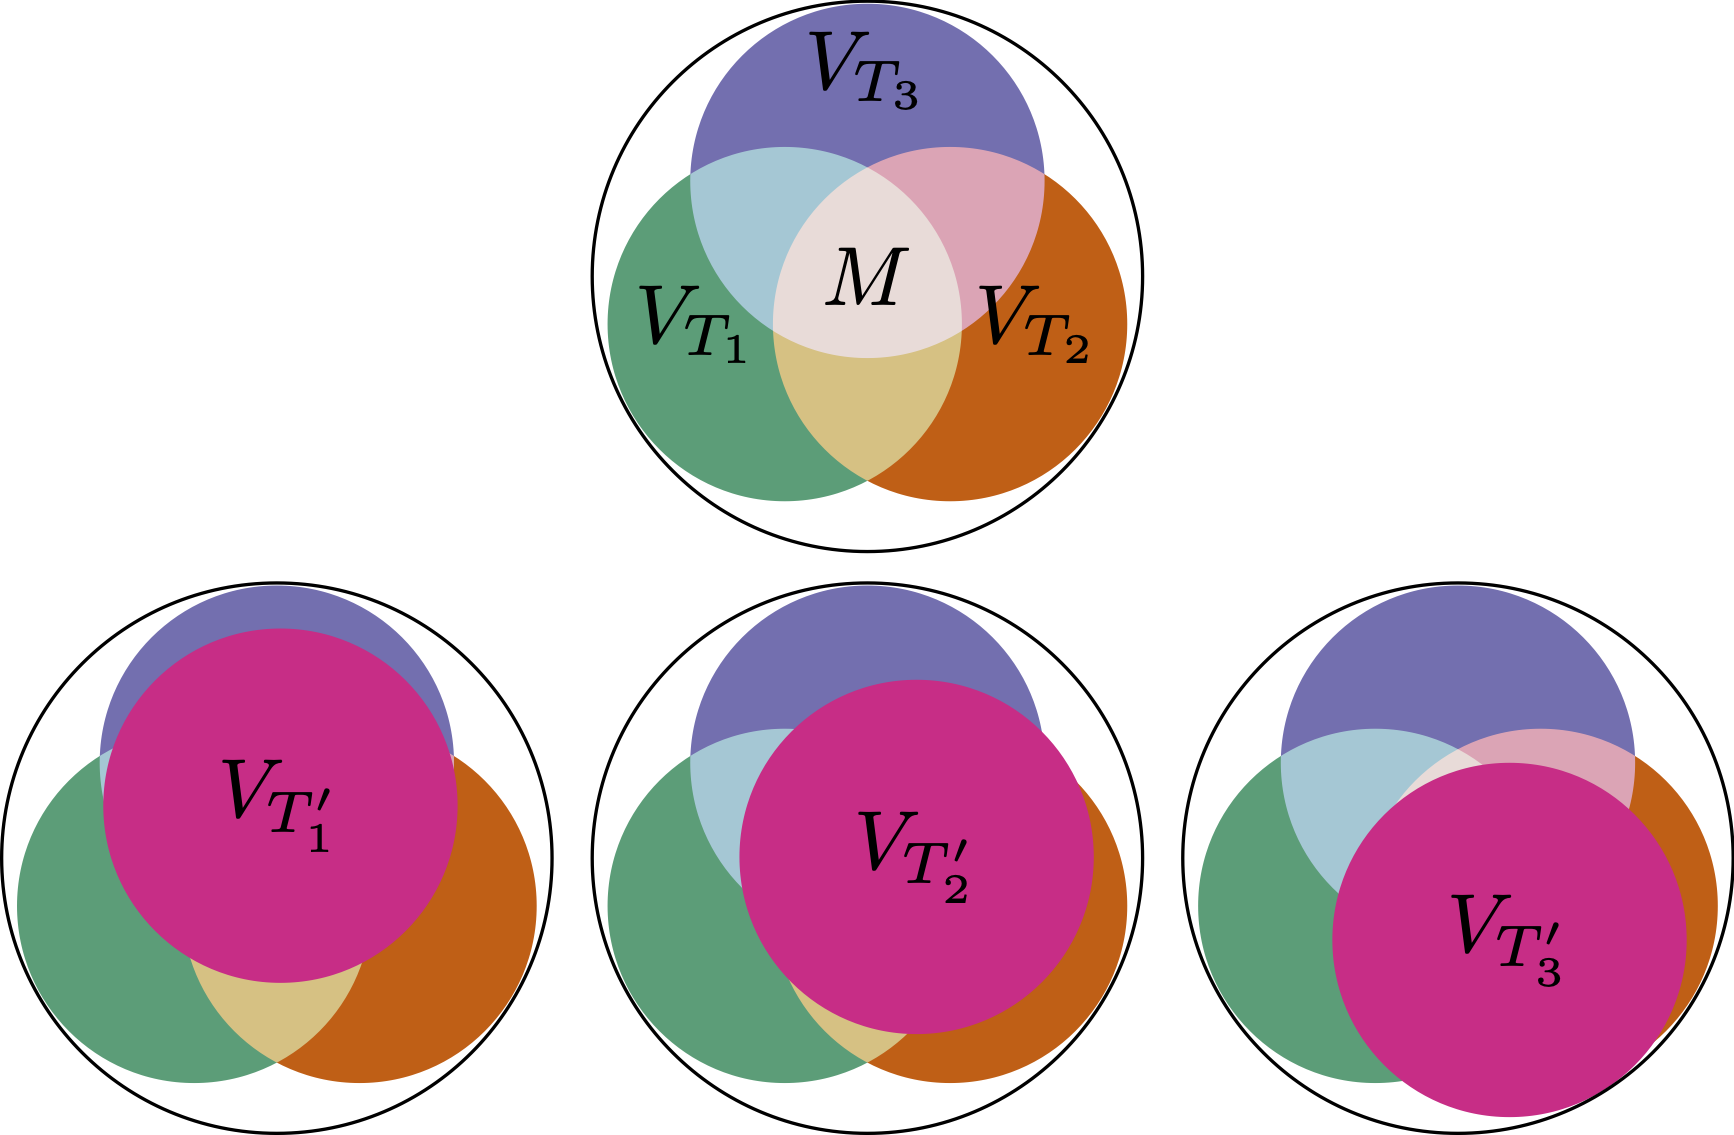
\includegraphics[width=0.95\linewidth]{img/robust_enum.png}
\caption{Conceptual visualization of how enumeration with diversity ensures robustness. The bounding circle represents the set of all nodes contained in any cheap relaxed Steiner tree. The sets $V_{T_i}$ represent the node sets of three pairwise diverse cheap relaxed Steiner trees. For any $\tau>2/3$, the set $M$ corresponds to the intersection of the sets $V_{T_i}$. The sets $V_{T_1^\prime}$ represent the node sets of three randomly sampled cheap relaxed Steiner trees. Nodes contained in $M$ are contained in almost all of the randomly sampled sets $V_{T_i^\prime}$.}
\label{fig:consensus}
\end{figure}

\subsection{Enumerating cheap and diverse relaxed Steiner trees}\label{sec:algo}
\todo[inline]{Dominik: This is just a first version that is supposed to give you an impression of what and how much there is to come. Will be polished as soon as I know more about the rest of the paper and can make it fit in nicely to the rest.}
% Idea
The primary idea of the algorithm is to compute prize-collecting steiner trees instead of normal steiner trees and lower the prizes of steiner points based on their usage to encourage the usage of other vertices.
A prize-collecting steiner tree does not have fixed terminals but instead every vertex has an individual prize that improves the objectives upon inclusion or equivalently penalises upon exclusion.
Normal steiner trees can be obtained by using high prizes for the terminals and zero prizes for all other vertices.
Computing prize-collecting steiner trees is NP-hard but a fast primal-dual algorithm with often nearly optimal solutions is known.
Because we do not want just one (nearly) optimal steiner tree but a diverse set, we add low prizes for non-terminal vertices that have a negligible influence on the optimal solution but are able, in case of multiple comparable solutions, to skew the odds in favour of specific solutions.
More precisely, we reduce the prizes of non-terminal vertices whenever they appear in a steiner tree.
This makes un- oder less used vertices more attractive and, hence, more likely to appear in a solution if they are actually good candidates.
Vertices that are not contained in any good steiner tree remain unattractive because the prizes are too low compared to the edge costs.

% Algorithm
Our proposed algorithm ROBUST is defined in \cref{alg:enum}.
Let $\textsc{PcstApx}(G,w,p)\rightarrow T$ be a prize-collecting steiner tree algorithm that recieves a graph $G=(V,E)$ with edge weight $w: E\rightarrow \mathbb{R}^+$ and prizes $p: V\rightarrow \mathbb{R}^+_0$, and returns a tree $T=(V_T, E_T), V_T\subseteq V$ that minimizes $\sum_{e\in E_T} w(e) + \sum_{v\in V\setminus V_T} p(v)$.
To make sure that all terminals are in the tree, we determine the prize $\gamma$ based on the diameter of the graph and the maximum edge weight. 
The prizes that are passed to \textsc{PcstApx} are defined by
\[v \mapsto \begin{cases} \gamma & \text{if }v\in S \\ \alpha\cdot \beta^{|\{T\in \mathcal{T} \mid v \in V(T)\}|} \cdot \min_{e\in E} w(e) & \text{else} \end{cases}\]
and decrease by a factor $\beta$ every time the corresponding non-terminal vertices are used, starting with $\alpha$ times the minimum edge weight.
\todo[inline]{Needs adaption as we no longer have strict steiner trees.}

\begin{algorithm}[h]
\SetAlgoLined
\KwIn{Graph $G=(V,E)$, edge weights $w: E\rightarrow \mathbb{R}^+$, terminals $S\subseteq V$, number of desired steiner trees $n\in \mathbb{N}$, parameters $\alpha\in \mathbb{R}^+$ and $\beta\in \mathbb{R}^+$}
\KwOut{Set of steiner trees $\mathcal{T}=\{T_1, T_2, \ldots, T_n\}$}
 $\mathcal{T} \gets \emptyset$\;
 $\gamma \gets \text{diam}(G)\cdot 2\cdot \max_{e\in E} w(e)$\;
 $i \gets 0$\;
 \While{$|\mathcal{T}|<n$}{
    $i \gets v \mapsto |\{T\in \mathcal{T} \mid v \in V(T)\}|$
    $p\gets v \mapsto \begin{cases} \gamma & \text{if }v\in S \\ \alpha\cdot \beta^{i(v)} \cdot \min_{e\in E} w(e) & \text{else} \end{cases}$\;
   $T=\textsc{PcstApx}(G, w, p)$\;
 }
 \Return $\mathcal{T}$
 \caption{$\mathtt{enumerate\_diverse}$}
 \label{alg:enum}
\end{algorithm}

% Used PCST algorithm
We use the primal-dual approximation algorithm of \cite{goemans1995general} and an implementation by \cite{hegde2015nearly}.
It has an guaranteed approximation factor of at most $2$ and a runtime complexity in $O(d |E| \log |V|)$ where $d$ refers to the encoding size in bits for the weight and prize values.
\cite{hegde2014fast} provide corresponding benchmarks.
The implementation is remarkably fast and solves instances with multiple hundreds of thousand edges within seconds (often even less than a second).

% Weight for terminals
We do not use very high prizes for the terminals because we cannot compute optimal prize-collecting steiner trees but only approximations.
The higher the prizes of the terminals is, the lower the influence of the edge weights and other prizes becomes but we are interested in those and not in the prizes of the terminals.
The guaranteed approximation factor, thus, could be bloated and weakened.
If the prizes of the terminals make up $\SI{50}{\percent}$ of the optimal objective value, the guaranteed approximation factor increases to $3$.
While the guaranteed approximation factor is only a worst-case upper bound and the actual solutions are often nearly optimal, it is still recommendable not to use unnecessarily high prizes.

% Min Edge Weight Problem
Using a fraction of the minimal edge weight works well if the edge weights are similar, best for uniform edge weights.
If the minimal edge weight is (nearly) zero, this approach fails.
By giving individual prizes based on the edge weights of incident edges, you could ease this problem.
When choosing the initial prizes, you have to make sure that they are not too high such that vertices become integrated just for their prizes but are actually bad for the steiner tree.
You also have to remember that the used algorithm is only an approximation algorithm and could, in worst-case, also choose bad vertices as long as they do not increase the objective by a factor greater than two.
Therefore, a small safety margin is advised.

% Alternative options
Instead of giving every non-terminal vertex an initial prize and lowering it, you can also start with zero-prizes and increase the prize every time the vertex is not in an solution.
However, this approach is harder to tune to make sure that good candidate become attractive enough but bad candidates not.
With our approach you only have to make sure, the initial value is properly chosen.

\section{Evaluation}

\subsection{Compared methods}

We compared ROBUST to the state-of-the-art DMMMs DIAMOnD \citep{diamond_ghiassian2015}, MuST \citep{covex_sadegh2020}, and DOMINO \citep{domino_levi2021}. These methods were selected for the following reasons: 
\begin{itemize}
\item They all expect binary input (\ie, lists of differentially expressed or disease-associated seed genes) and are hence directly comparable to our method ROBUST.
\item DOMINO has been shown to outperform other DMMMs in two independent studies \citep{domino_levi2021,amim_lazareva2021} and can hence be considered to be one of the best available methods.
\item Based on the number of citations, DIAMOnD is arguably one of the most widely used DMMMs.
\item MuST constituted the point of departure for the development our new method ROBUST and also models disease modules via Steiner trees.
\end{itemize}

Moreover, we compared ROBUST to a na\"ively implemented baseline, where instead of enumerating diverse prize-collecting Steiner trees as detailed in \Cref{alg:robust}, we enumerate multiple close-to-optimal Steiner trees by simply shuffling the input data and running the classical $2$-approximation algorithm by \cite{kou:1981aa} several times. In the sequel, this na\"ive implementation is called R-MuST (randomized MuST). Details about the non-deterministic steps in all compared methods can be found in the supplement. 

Both ROBUST and R-MuST return a set of k Steiner trees $\mathcal{T}_k^G = (T_i^G)_{i=1}^k$ with $T_i^G=(V_i^G, E_i^G)$ for a network $G=(V,E)$. For our evaluation, k was set to 10. Given a threshold $\tau \in (0,1]$, we define the solution node set \begin{equation}
    V_{k, \tau}^G := \bigg\{ v \in V: \sum_{i=1}^k[v \in V_i^G] \geq \tau \cdot k \bigg\}
\end{equation}
as the set of nodes that appear in at least $100 \cdot \tau \%$ of the Steiner trees contained in $\mathcal{T}_k^G$.  

\subsection{Robustness tests}

\subsubsection{Protocol and data used for robustness tests}

The methods were tested on a human PPI network obtained from IID \citep{iid_kotlyar2019}, filtered based on experimental validation. The network therefore consists of \num{329215} edges between \num{17666} proteins. Sets of disease-associated seed genes were constructed for \num{903} disease by merging the disease-gene associations from OMIM \citep{Amberger2019-mp} and DisGeNET \citep{disgenet_pinero2020} and then removing sets with more than twenty genes. Running the tests on larger seed sets was not feasible due to the high runtimes of both MuST and R-MuST.

Robustness was measured as follows: Each tested DMMM \ALG was run twenty times on each seed set $S$. In each iteration, the input PPI network was randomly permuted before running \ALG, yielding twenty disease modules. Let $M^{\ALG,S}_i$ be the node set of the $i^\text{th}$ disease module computed by \ALG on $S$. Then we quantified \ALG's robustness on $U$ using the mean Jaccard index
\begin{equation*}
r_S(\ALG) \coloneqq\binom{20}{2}^{-1} \sum_{i=1}^{19} \sum_{j=i+1}^{20} \frac{|M^{\ALG,S}_i \cap M^{\ALG,S}_j|}{|M^{\ALG,S}_i \cup M^{\ALG,S}_j|}\text{,}
\end{equation*}
\ie, $r_S(\ALG)\in[0,1]$ and large values of $r_S(\ALG)$ indicate that \ALG is robust to random storage order on the seed set $S$.

ROBUST was run with an initial fraction value of 0.25 and a reduction factor of 0.9. All hyper-parameters of the competitor methods were set to the default values.

\subsubsection{Effect of hyper-parameters on robustness}

\subsubsection{Robustness in comparison to competitors}

\begin{figure*}[htb]
\centering
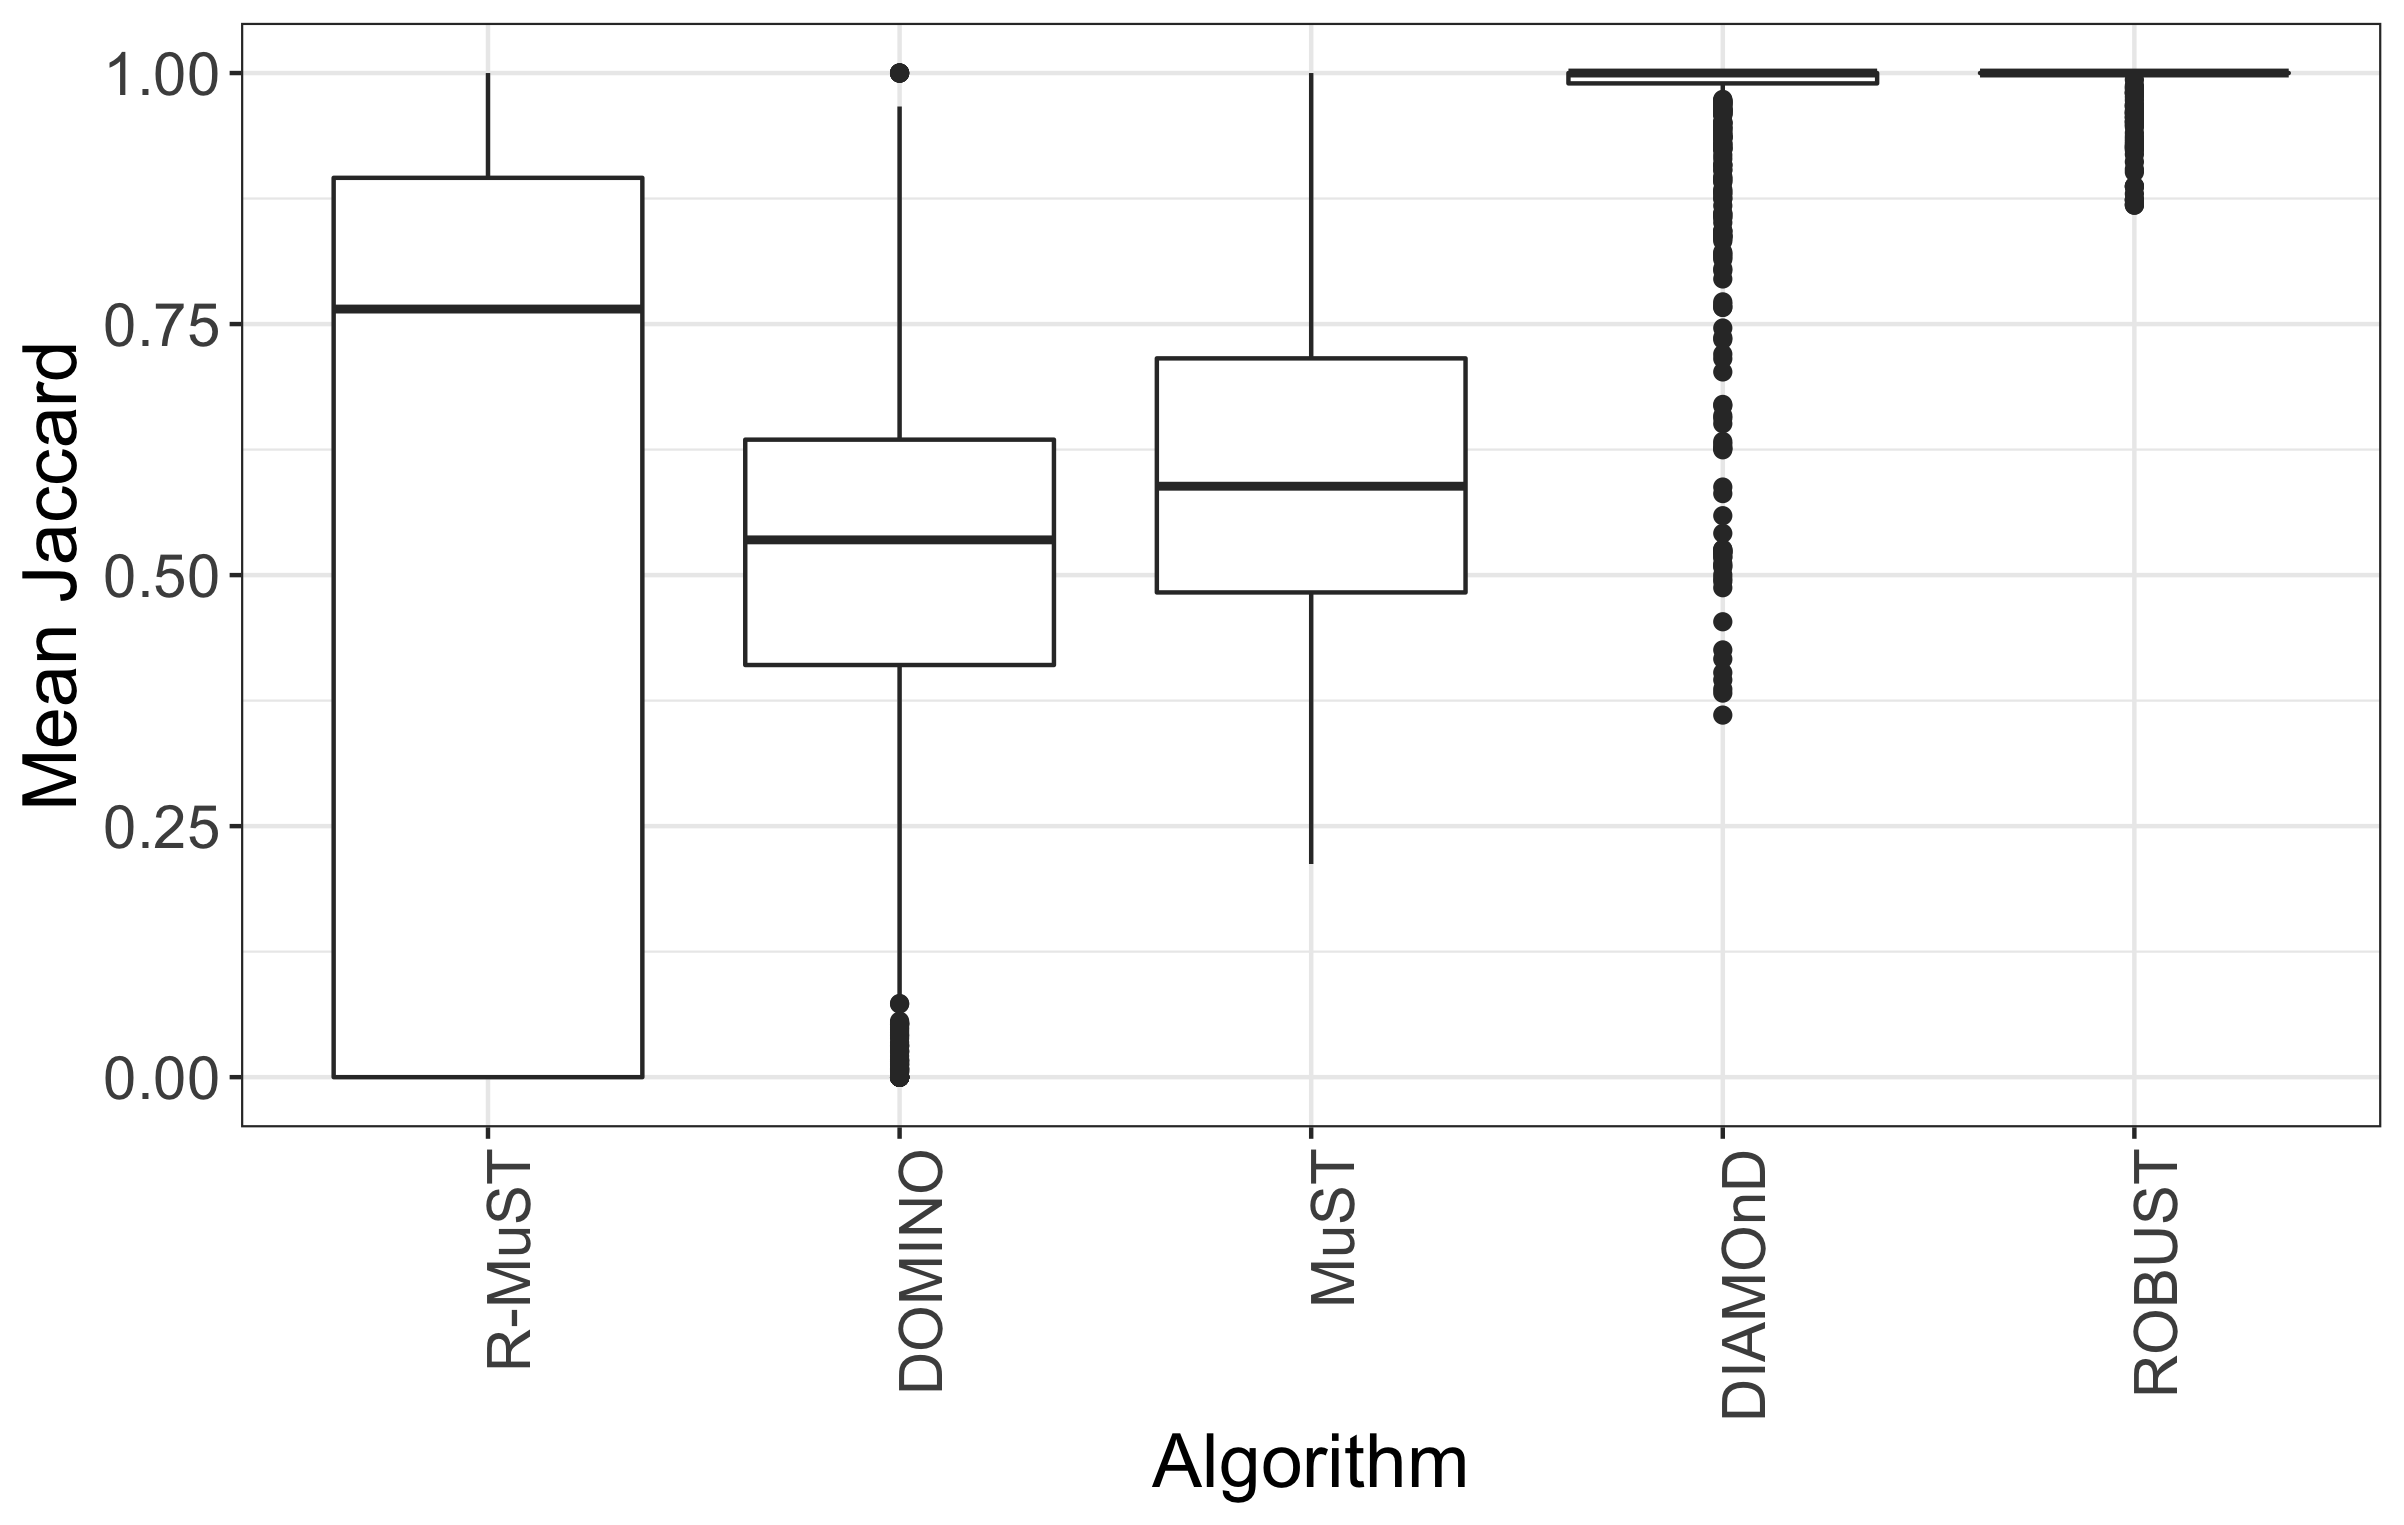
\includegraphics[width=0.8\linewidth]{img/all_robustness_results.png}
\caption[Robustness in comparison to competitors.]{Robustness in comparison to competitors tested on 903 disease-associated seed genes projected on the IID network. ROBUST performs superior to its precursors MuST and R-MuST and achieves almost perfect robustness. DIAMOnD yields solutions that are more robust than the DOMINO solutions but both methods are outperformed by ROBUST. The results of R-MuST vary strongly, especially for higher thresholds. For ROBUST, higher thresholds yield more stable solutions.}
\label{robustness_subset}
\end{figure*}

Figure \ref{robustness_subset} shows the distribution of the 903 mean Jaccard indices for each of the methods. It is clearly visible that the implementation of ROBUST is superior to its precursors MuST and R-MuST. While the robustness increases for ROBUST for higher threshold values, the opposite can be observed for R-MuST. In fact, the R-MuST results vary so strongly that we decided to leave the algorithm out when comparing functional relevance. DIAMOnD is more robust than DOMINO but ROBUST yields significantly higher mean jaccard indices than both methods (see Supplementary Table xxx) and achieves almost perfect robustness. 

\subsection{Functional relevance tests}

\subsubsection{Protocol and data used for functional relevance tests}

Functional relevance tests were conducted by implementing custom wrappers for the AMIM test suite introduced by \cite{amim_lazareva2021}. In the test suite, gene expression datasets with case/control information for five complex diseases are used, namely amyotrophic lateral sclerosis (ALS), non-small cell lung cancer (LC), ulcerative colitis (UC), Chron's disease (CD) and Huntingtons disease (HD). The seed genes were obtained by applying a two-sided Mann-Whitney U-test on the case/control expression vectors and extracting all genes with a p-value smaller than $0.001/n$. Each set of seed genes was projected onto one of the five widely used PPI networks BioGRID (\cite{biogrid_oughtred2019}), APID (\cite{apid_alonso2016,apid_alonso2019}), STRING (\cite{string_szklarczyk2019}) with high confidence interactions only, HPRD (\cite{hprd_keshava2009}) and IID (\cite{iid_kotlyar2019}). Since we were only interested in the functional relevance results on the real dataset, none of the network generators of the test suite were used. 

Functional relevance was evaluated by computing gene set enrichment using the KEGG pathways (\cite{kegg_kanehisa2016}) corresponding to the diseases and by computing overlap coefficients with the disease-associated DisGeNET (\cite{disgenet_pinero2020}) gene sets. For more detailed information, please refer to \cite{amim_lazareva2021}.

\subsubsection{Functional relevance in comparison to competitors}

\begin{figure*}[htb]
\centering
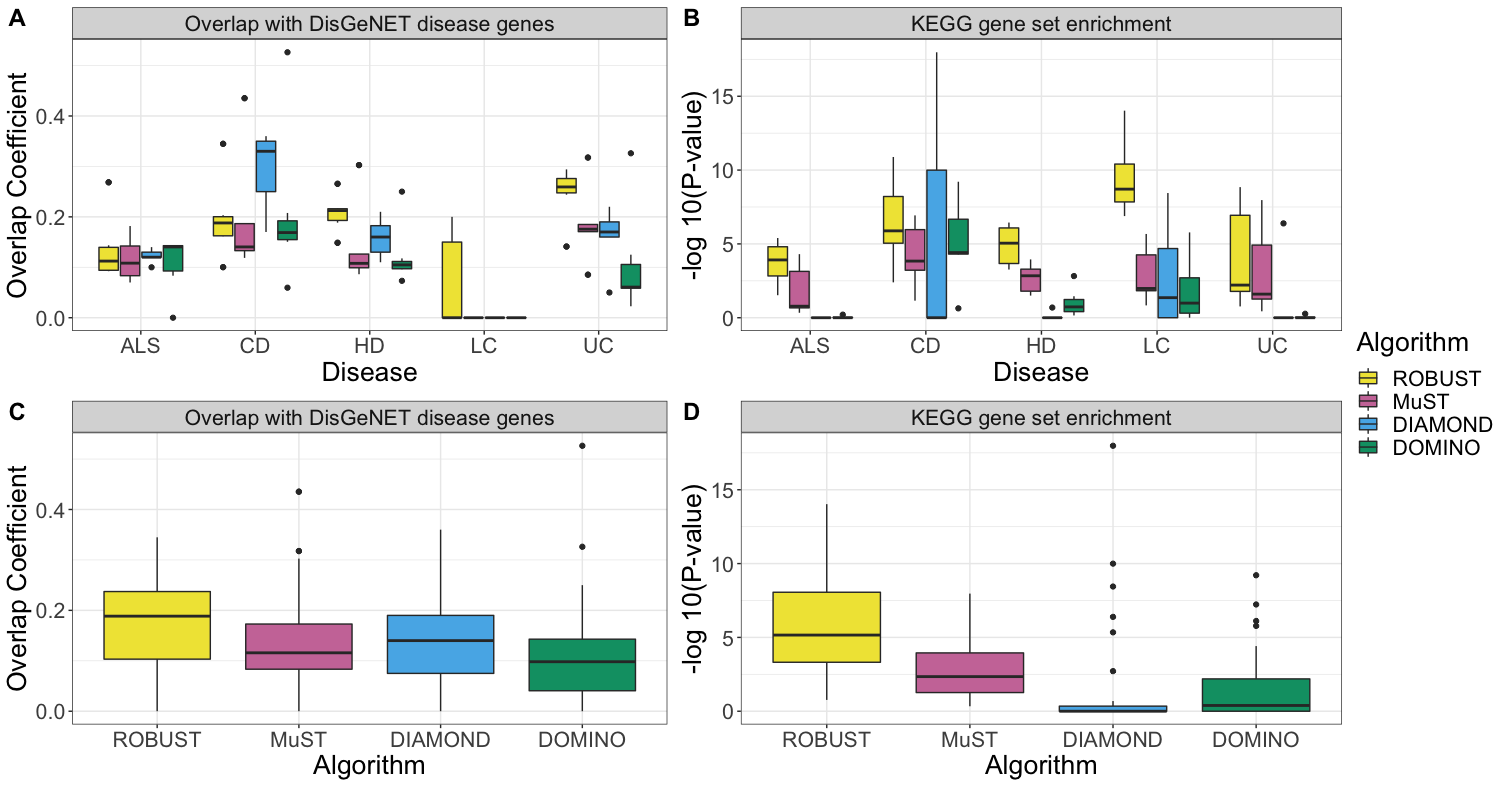
\includegraphics[width=0.95\linewidth]{img/functional_relevance_all.png}
\caption[Distribution of the functional relevance scores.]{Distribution of the functional relevance scores for ROBUST, MuST, DIAMOnD and DOMINO run on the five disease networks. \textbf{A}: Overlap coefficient of the solution set and the DisGeNET disease genes, split by disease. \textbf{B}: KEGG gene set enrichment P-values splot by disease. \textbf{C}: Overlap coefficient distribution over all networks and disease seed sets. \textbf{D}: KEGG gene set enrichment distribution over all networks and disease seed sets.}
\label{functional_relevance}
\end{figure*}

Figure \ref{functional_relevance} shows the distributions of the functional relevance scores for ROBUST, MuST, DIAMOnD and DOMINO run on the five disease networks. In Figure \ref{functional_relevance}A and B the overlap with DisGeNET disease genes and the KEGG gene set enrichment is shown for each disease while Figure \ref{functional_relevance} C and D contains the score distributions concatenated over all five diseases. Overall, ROBUST outperforms the other three algorithms, especially for the LC seeds. The CD dataset is the only case where DIAMOnD yields better results than ROBUST.   

\section{Case study for [NAME OF DISEASE]}

%Case study for hereditary ovarian cancer: In order to show that ROBUST is able to infer biologically meaningful information, we performed a case study for hereditary ovarian cancer. First, the PPI network was obtained from IID and filtered for experimentally validated interactions. Because context-specific networks are very helpful for reducing the false positive rate, the IID network was subsetted to only contain interactions measured in ovarian tissue. Then, a set of 14 seed genes (and their corresponding proteins) for hereditary ovarian cancer was obtained from DisGeNet (ID: C1333992). 
%ROBUST was run with an initial fraction of 0.25 and a reduction factor of 0.9. In the 10 trees that were computed, Annexin A7 (P20073), Syndecan-1 (P18827), CD44 antigen (P16070) and the cytosolic Thymidine kinase (P04183) were found five times. Poly(rC)-binding protein 1 (Q15365) and Partitioning defective 3 homolog (Q8TEW0) occurred four times.  

\section{Discussion}


\section*{Acknowledgements}


\section*{Funding}


\bibliographystyle{natbib}
\bibliography{references}
\end{document}
